% ! TeX root = ../thesis-main.tex
%----------------------------------------------------------------------------------------
\chapter{Analysis}
\label{chap:analysis}
%----------------------------------------------------------------------------------------
This chapter defines the scope, requirements, and use cases of \this, based on the expectations of the stakeholders, consisting of ScaFi developers and researchers.
%
A priority analysis is conducted using the MoSCoW method, ensuring that the work stays focused on delivering key features while meeting technical constraints and user preferences.

\section{Requirements analysis} \label{chap:analysis->sec:requirement-analysis}

Since the very beginning, \this aimed to redesign ScaFi using Scala 3 to improve the quality of the code, including but not limited to readability, maintainability, and reusability.
%
This time, the implementation is based on \ac{XC} as the theoretical foundation, through which the \ac{FC} constructs could be implemented.

The project started interviewing the stakeholders, including developers and researchers who developed the original ScaFi and still use it, in order to understand their needs and expectations.

The \textit{key users} identified for the library are:
\begin{itemize}
    \item \textit{End users}, that are the developers who will use the library to implement their aggregate programs;
    \item \textit{Library developers}, who will extend the library with new features, constructs, and syntax;
    \item \textit{Researchers}, who will experiment with the calculus foundations and could benefit from reusing existing libraries.
\end{itemize}

During the stakeholder interviews, a comprehensive list of functional and technical requirements emerged, which were then carefully curated and prioritized through extensive discussions and feedback sessions.

\paragraph{Functional requirements} are the features that the library must provide to the users. The following are the most relevant functional requirements identified:
\begin{enumerate}[label=\textbf{F.\arabic*}]
    \item redesign and implement a new \ac{API} for the \texttt{core} package\Cref{chap:analysis->sec:scafi-analysis};
    \item redesign and implement the \texttt{tests} package with acceptance tests, easy to read and understand, and that can be used as examples;
    \item use the \ac{XC} as the foundation of the (default) implementation of constructs, while still providing a \ac{FC} based API;
    \item develop an \textit{Alchemist incarnation}\footnote{\url{https://github.com/AlchemistSimulator/Alchemist}}~\cite{alchemist}, enabling \this programs to run on the well-tested and widely used Alchemist simulator;
    \item develop a minimal, pure Scala 3 simulator to run tests and examples without the need for external dependencies;
    \item provide a new API for the \texttt{core} package that allows developers to import arbitrary ScaFi libraries and constructs into their programs without conflicts, in a seamless way;
    \item prefer keeping the original, abbreviated names for core constructs like \texttt{nbr} and \texttt{rep}, as they are widely adopted and recognized within the community, promoting consistency and familiarity;
    \item conduct experiments with Scala 3 to explore and achieve new compile time features for ScaFi, to enhance code quality and elevate the overall user experience.
\end{enumerate}

\paragraph{Technical requirements} are the constraints and guidelines that the library must follow to ensure the quality of code and user experience.
\begin{enumerate}[label=\textbf{T.\arabic*}]
    \item use Scala 3 as the host language to leverage its advanced features and enhancements;
    \item enable quality options on the Scala 3 compiler such as explicit nulls (\Cref{chap:background->sec:scala3->subsec:explicit-nulls}) and multiversal equality (\Cref{chap:background->sec:scala3->subsec:multiversal-equality});
    \item employ \ac{SBT} as build system;
    \item cross-build the project for \textit{scala-js}\footnote{\url{https://www.scala-js.org}};
    \item cross-build the project for \textit{scala-native}\footnote{\url{https://scala-native.org}};
    \item lint the code with \textit{scalafix}\footnote{\url{https://scalacenter.github.io/scalafix}} and/or \textit{scalafmt}\footnote{\url{https://scalameta.org/scalafmt}};
    \item avoid using third-party libraries for the \texttt{core} package dependencies.
\end{enumerate}

Following the identification of requirements, a comprehensive discussion and prioritization process was undertaken, guided by the \ac{MoSCoW} method.
%
The results are outlined in detail in Table \ref{tab:requirements-prioritization}.

\begin{table}[ht]
\centering
\caption{Requirements prioritization.}
\label{tab:requirements-prioritization}
\begin{tabular}{|>{\hspace{0pt}}m{0.362\linewidth}|>{\hspace{0pt}}m{0.277\linewidth}|>{\hspace{0pt}}m{0.238\linewidth}|} 
    \hline
    \textbf{Requirement} & \textbf{MoSCoW} & \textbf{Priority}  \\ 
    \hline
    F.1          & must   & high      \\ 
    \hline
    F.2          & must   & high      \\ 
    \hline
    F.3          & must   & high      \\ 
    \hline
    F.4          & could  & low       \\ 
    \hline
    F.5          & must   & high      \\ 
    \hline
    F.6          & should & average   \\ 
    \hline
    F.7          & should & average   \\ 
    \hline
    F.8          & won't  & low       \\ 
    \hline
    T.1          & must   & high      \\ 
    \hline
    T.2          & should & high      \\ 
    \hline
    T.3          & must   & high      \\ 
    \hline
    T.4          & could  & low       \\ 
    \hline
    T.5          & could  & low       \\ 
    \hline
    T.6          & should & low       \\ 
    \hline
    T.7          & should & average   \\
    \hline
\end{tabular}
\end{table}

Finally, before starting with the design of the solution, given that the project is a redesign of an existing library, the requirements were compared with the existing ScaFi library to identify the differences and similarities.

\section{ScaFi} \label{chap:analysis->sec:scafi-analysis}

The ScaFi repository\footnote{\url{https://github.com/scafi/scafi}} is organized in modules, as illustrated in \Cref{fig:scafi-project-org}.
%
For most of the use cases, only a small subset of the modules should be imported.
%
The \this project primarily focuses on redesigning and implementing the \texttt{core} package, implicitly including \texttt{commons} module, as well as the \texttt{simulator} and \texttt{tests} packages.
%
However, it should be noted that the simulator implementation planned for this project will be a minimal version written in pure Scala 3, as opposed to the existing \texttt{simulator} module, which is a complex and feature-rich suite of tools for simulating aggregate programs in space and time.
%
Porting the remaining modules, which encompass various \ac{GUI} implementations, demos, and integration with \textit{Akka}\footnote{\url{https://akka.io}} for actual deployment of real-world aggregate applications, is out of the scope of \this, and will be addressed in \Cref{chap:conclusion-and-future-work}.

\begin{figure}
    \centering
    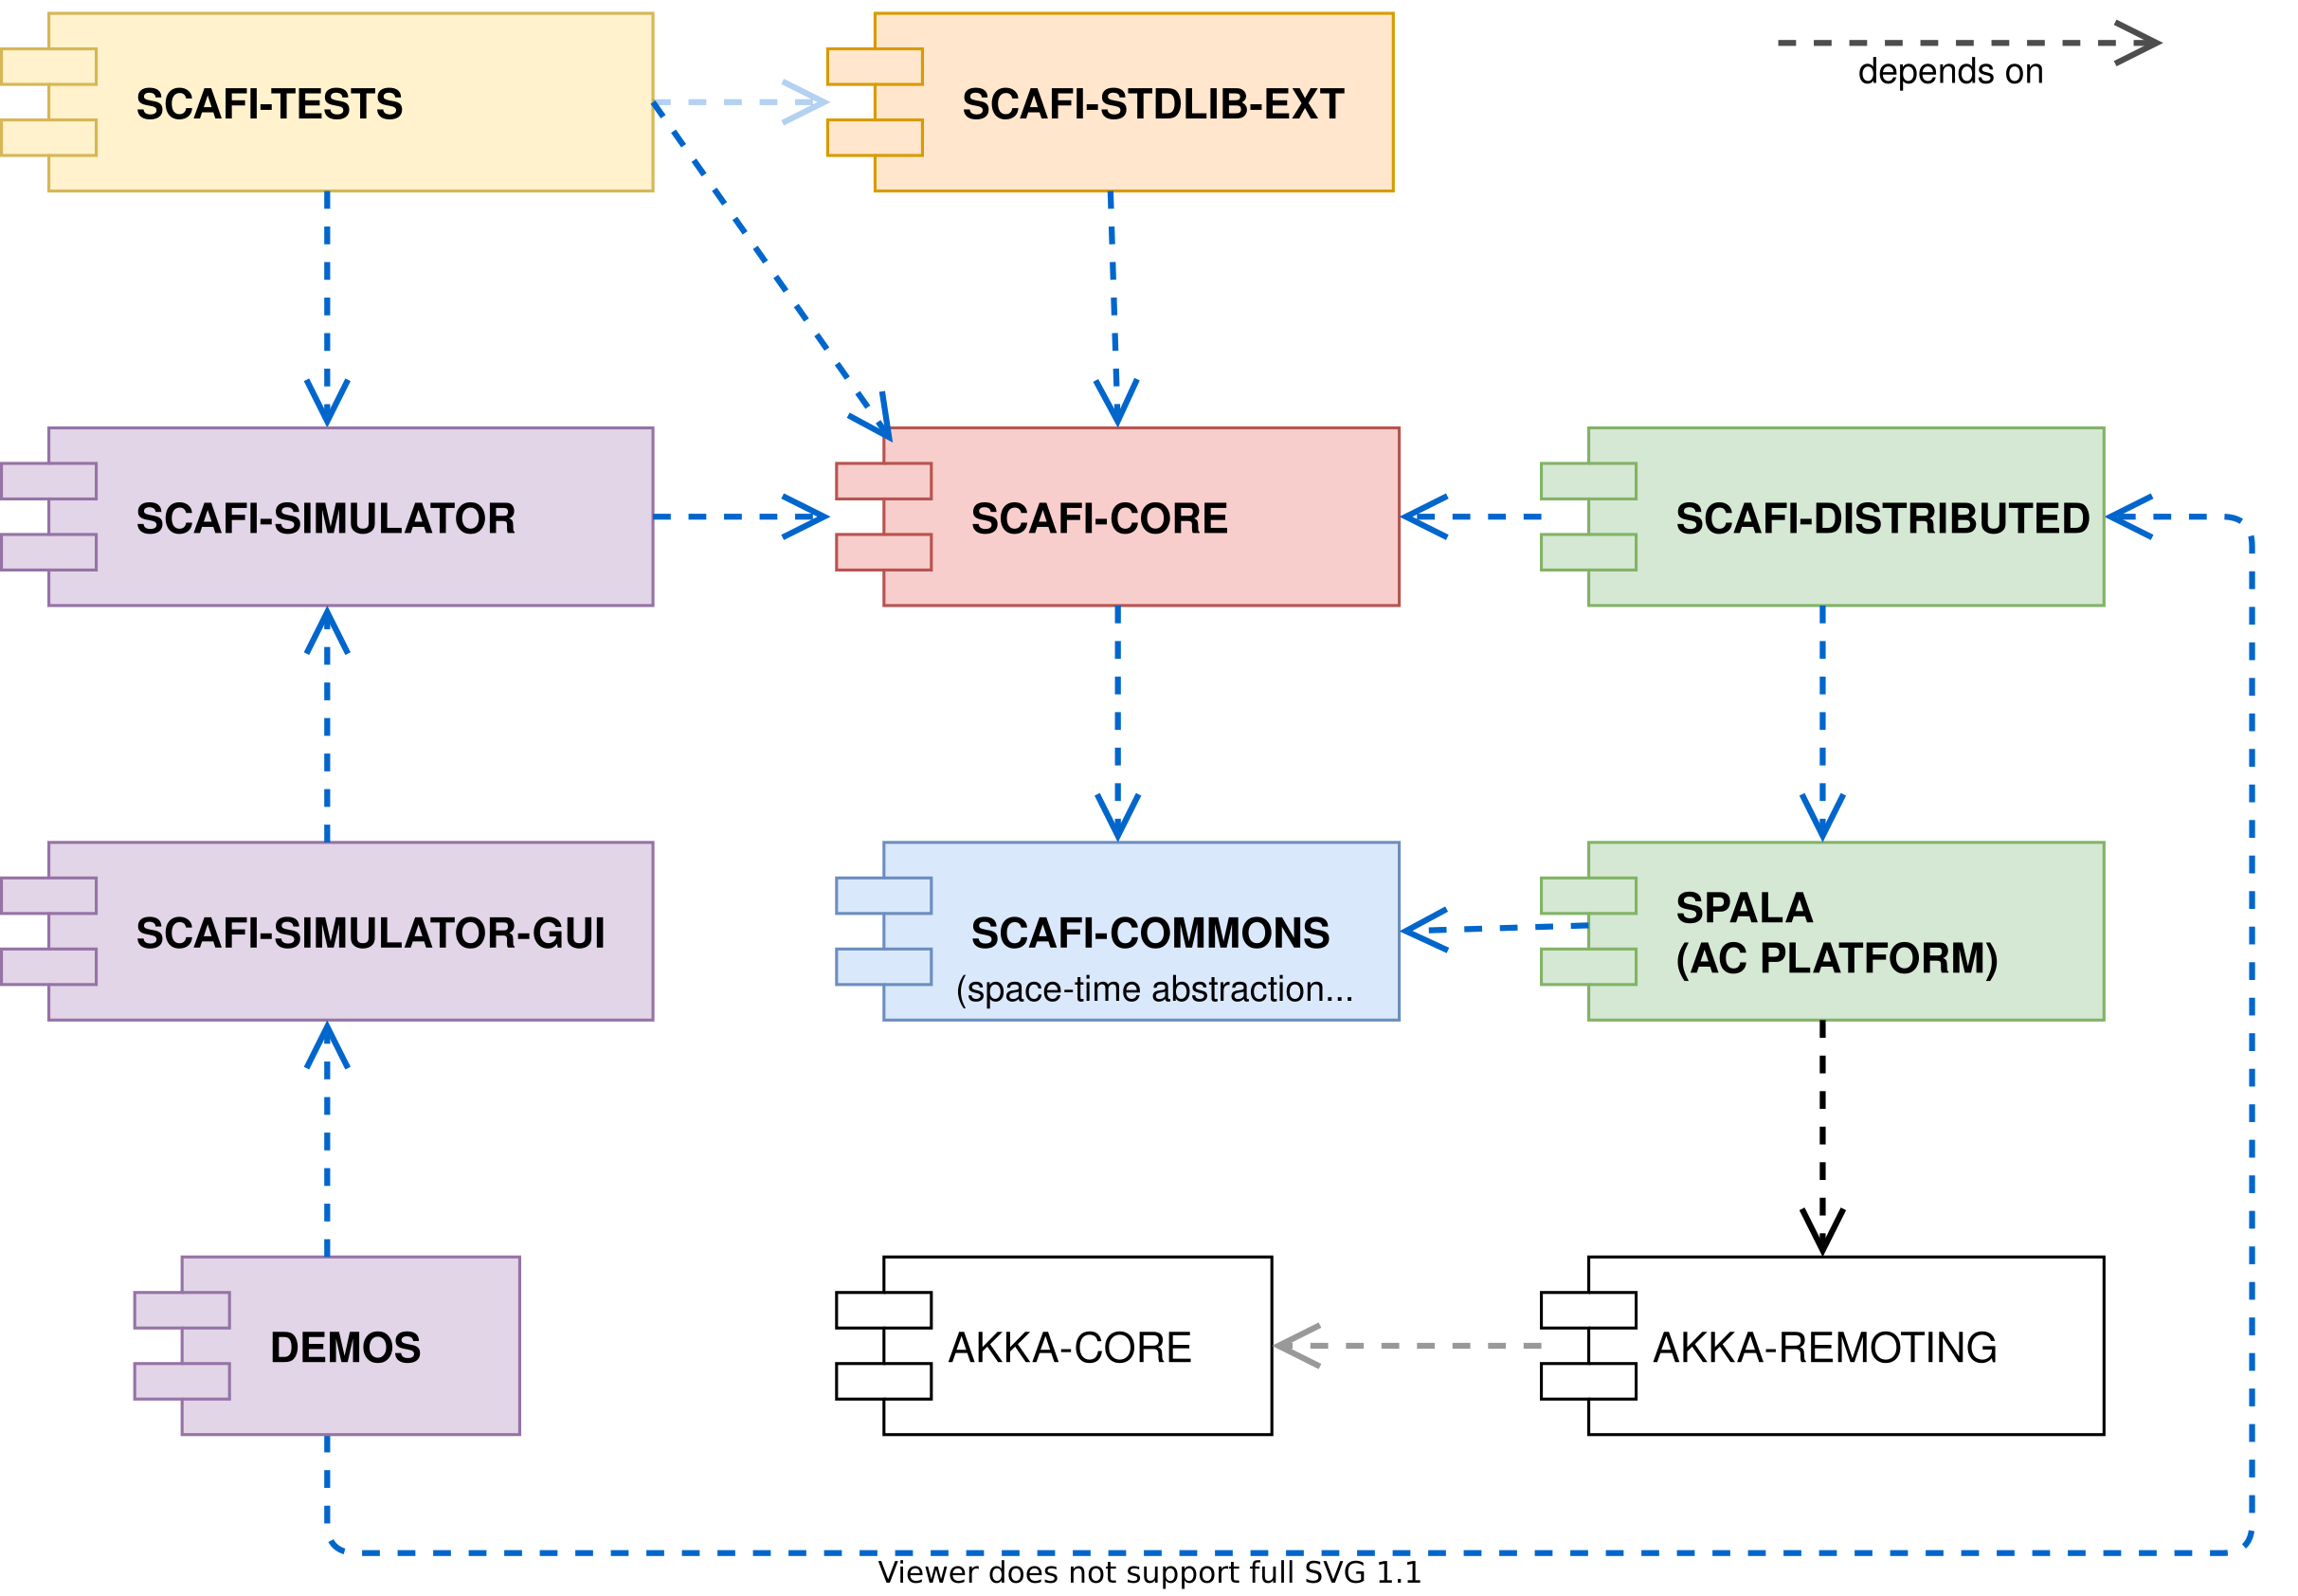
\includegraphics[width=.8\linewidth]{figures/scafi-project-org.drawio.png}
    \caption{ScaFi project organization.}
    \label{fig:scafi-project-org}
\end{figure}

Within the \texttt{core} package of the \texttt{core} module, the \texttt{Core} trait serves as the root of the family of traits.
%
It defines the set of abstract type members and traits, such as \texttt{Context}, that represents the context of the aggregate program execution.
%
A trait \texttt{Language} defines a \texttt{Constructs} trait with the core syntax of \ac{FC}, such as \texttt{rep}, \texttt{nbr}, and \texttt{foldhood}, plus additional utilities such as \texttt{mid(): ID} for retrieving the device own identifier and \texttt{sense[A](name: CNAME): A} for sensing a value from the environment.
%
Furthermore, the \texttt{RichLanguage} trait extends \texttt{Language} with additional constructs, such as \texttt{branch}, \texttt{foldhoodPlus}, and \texttt{maxHood}.
%
The \texttt{Semantics} trait implements the \ac{FC} constructs, the value tree building, and the \textit{foldhood context semantics}.
%
More insights on the foldhood semantics are provided in \Cref{chap:analysis->sec:scafi-analysis->subsec:foldhood-semantics}.
%
In addition to that, the \texttt{core} module contains other packages, such as \texttt{lib} offering standard libraries, and the utilities to provide a fully-fledged aggregate program execution environment called \textit{incarnation}.
%
The \texttt{distributed} and \texttt{spala} modules enable ScaFi to run on real-world distributed applications by leveraging integration with the \textit{Akka framework}\footnote{\url{https://akka.io}} and with other supportive libraries such as \textit{Java Swing} and the \textit{Play Framework}\footnote{\url{https://www.playframework.com}}.
%
Lastly, the \texttt{simulator} and affiliated modules provide an advanced simulation suite featuring spacial and temporal simulation alongside multiple \ac{GUI} options, including a tridimensional renderer.

To use a library component in ScaFi, the user must mix in the library trait with the \texttt{AggregateProgram} base class, as shown in \Cref{lst:using-libraries-in-scafi}.
%
As a consequence, all the transitive dependencies of the mixed-in libraries become visible within the scope of the program, necessitating careful construction of libraries to avoid conflicts.

\lstinputlisting[float, language=Scala, caption={Using a library component in ScaFi.}, label={lst:using-libraries-in-scafi}]{listings/scafi-using-libraries.scala}

Once the program is defined within the \texttt{main} method of the \texttt{AggregateProgram} extension, the user can execute the program on the simulator through the \texttt{Launcher}.
%
This specialized extension of Scala's \texttt{App} trait provides a \texttt{launch} method to start the simulation with one of the available \acp{GUI}.

\this aims to redesign and implement the \texttt{core} package to maintain the feasibility of integrating an equally sophisticated simulation suite while improving the overall quality of the code and the user experience.

\subsection{Foldhood semantics in ScaFi} \label{chap:analysis->sec:scafi-analysis->subsec:foldhood-semantics}

ScaFi employs the concept of a stateful \quotes{virtual machine} as its core to monitor the context of expression evaluation within the aggregate program.
%
The virtual machine not only tracks nested invocations of core constructs, but also the scope of foldhood expressions.
%
These are evaluated for each neighbor of the device, and the results of the evaluations are combined into a single value.
%
By adopting this approach, ScaFi avoids the definition of an explicit type for fields, resulting in a clean syntax but leaving the awareness of the underlying field-like nature of the foldhood semantics to the user.
%
For instance, the invalidity of expressions like \texttt{nbr{nbr{x}}} within a foldhood is something that the user must be aware of, as it is not enforced by the compiler or the virtual machine.
